\documentclass[reprint, aps, prl, amsmath, amssymb, showkeys]{revtex4-2}

\usepackage{xcolor}
\usepackage{soul}
\usepackage{newtxtext}
\usepackage[cmintegrals]{newtxmath} 
\usepackage{graphicx}
\usepackage{hyperref}
\usepackage{cleveref}
\hypersetup{colorlinks,
	linkcolor={blue!75!black!80!yellow},
	citecolor={blue!75!black!80!yellow},
	urlcolor={blue!75!black!80!yellow}
}

\usepackage{algorithm} 
\usepackage{algpseudocode}

\begin{document}

\title{
The ABCs of Phase Retrieval:\\
Connecting the Acronyms of Scanning Transmission Electron Microscopy
}
\author{Georgios Varnavides}
\email{g.varnavides@tudelft.nl}
\affiliation{
Department of Imaging Physics, Delft University of Technology, Lorentzweg 1, 2628 CJ Delft, The Netherlands
}
\author{Willem P.M. de Kleijne}
\affiliation{
Department of Imaging Physics, Delft University of Technology, Lorentzweg 1, 2628 CJ Delft, The Netherlands
}
\author{Stephanie M. Ribet}
\email{sribet@lbl.gov}
\affiliation{
National Center for Electron Microscopy, Molecular Foundry, Lawrence Berkeley National Laboratory, Berkeley, CA 94720, USA
}

\begin{abstract}
High-resolution scanning transmission electron microscopy (STEM) is an indispensable tool for characterizing the structure and properties of materials down to the atomic scale.
Conventional STEM imaging, however, is limited by the phase problem, whereby the phase of the electron exit wave is lost upon detection.
Recent advances in diffractive imaging and 4D-STEM have enabled a range of phase retrieval techniques that computationally reconstruct the missing information.
These approaches offer improved dose efficiency and enhanced  sensitivity to weakly scattering signals, extending quantitative imaging to beam-sensitive materials composed of light elements.
In this work, we introduce the phase problem in electron microscopy and survey the diverse landscape of phase retrieval techniques used in the field.
Despite their many acronyms and algorithmic variations, these techniques share a common physical and mathematical foundation.
We present a unified framework that connects these seemingly distinct methods, from parallax imaging and tilt-corrected bright field (tcBF-STEM), to aberration-corrected bright-field (acBF-STEM), optimum bright field (OBF-STEM) and single-sideband (SSB) ptychography, as well as iterative ptychographic algorithms.
Based on these insights, we discuss the opportunities and practical limitations of applying these methods across different materials systems, detector designs, and microscope configurations.
\end{abstract}

\keywords{transmission electron microscopy (TEM); scanning transmission electron microscopy (STEM); nanostructure; crystallographic structure; 2D materials}

\maketitle

\section{Introduction}

Scanning transmission electron microscopy (S/TEM) enables the characterization of specimens from the micron scale down to the atomic scale, making it an indispensable characterization tool for any materials scientist~\cite{Williams_2009}.
S/TEM instruments operate in two complimentary acquisition modalities: \emph{imaging mode}, which produces a magnified real-space image of the specimen, and \emph{diffraction mode}, which records the angular distribution of scattered electrons in reciprocal space~\cite{Carter_2016}.

Traditional parallel-illumination TEM imaging is widely used across disciplines, from high-resolution studies of frozen-hydrated biomolecules~\cite{Vinothkumar_2016} to lattice-resolved~\cite{Alcorn_2023} and defect~\cite{Fultz_2013} imaging of materials.
In contrast, STEM employs a highly converged electron probe containing a broad range of incident wavevectors. 
When this probe interacts with the specimen, it produces a diffraction pattern that encodes the local scattering. 
In this sense, STEM is inherently a diffraction-mode technique, although real-space images can be obtained by processing the resulting position-resolved diffraction patterns -- a process we will refer to as \emph{diffractive imaging}.
This approach routinely provides interpretable, atomic-resolution imaging of crystalline materials and forms the basis of modern materials characterization~\cite{Ophus_2023}.

Both modalities are fundamentally limited by the microscopy ``phase problem,'' first recognized in quantum scattering by Max Born~\cite{born1926quantenmechanik} and discussed in his Nobel Lecture~\cite{born1954}.
Here, we focus on the mathematical foundations of STEM phase-retrieval techniques, which reconstruct the missing phase and thereby overcome these intrinsic contrast limitations.
We emphasize the implications of these methods for quantitative materials characterization and set the stage for a unified treatment of the underlying physics.

\begin{figure*}[t]
  \centering
  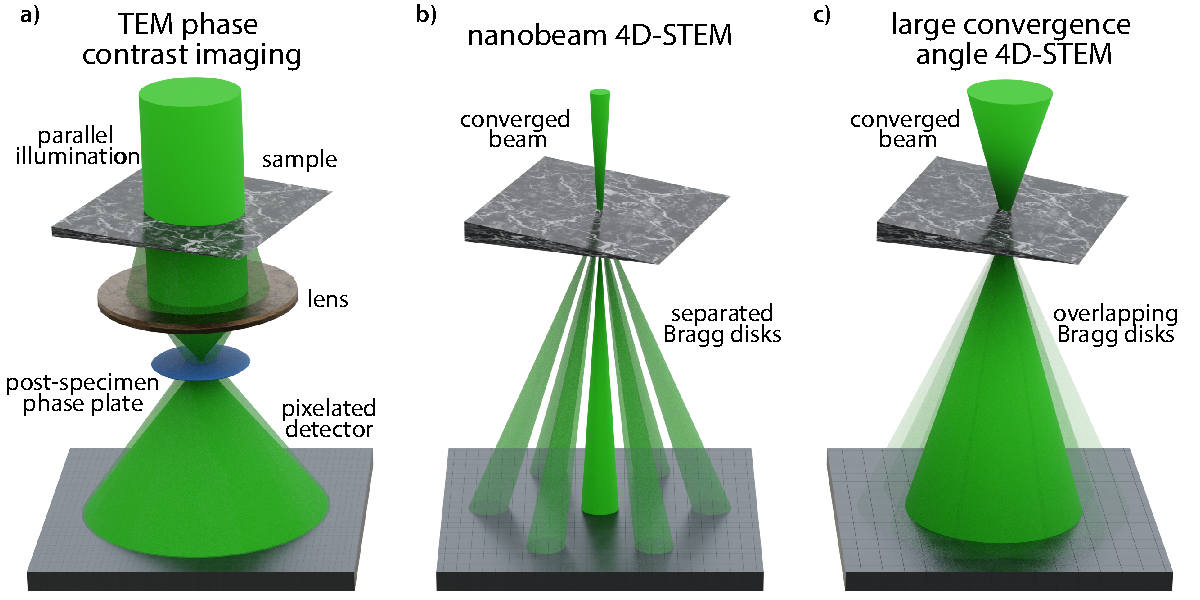
\includegraphics[width=\textwidth]{vector/schematic.pdf}
  \caption{Microscope configurations.
  (a)~TEM Zernike phase-contrast imaging,
  (b)~small-convergence-angle 4D-STEM, used for ``nanobeam'' experiments,
  and (c)~large-convergence-angle 4D-STEM, used for diffractive imaging experiments.}
  \label{fig:schematic}
\end{figure*}

\subsection{Microscopy Phase Problem}

The phase problem arises in electron microscopy because the scattered electron wavefunction -- the ``exit wave'' -- is complex-valued, yet physical detectors only measure real-valued intensities~\cite{Fienup_1982}.
In other words, although the specimen primarily imprints a \emph{phase shift} on the complex incident electron wavefunction $\psi$, the detector records $|\psi|^2$, seemingly discarding the information that carries most of the specimen's structure~\cite{born1954}.

For S/TEM, this becomes clear in the wave propagation formalism.
The evolution of an electron wavefunction, $\psi(\boldsymbol{r})$, along the optical axis $z$ is governed by the Schr\"odinger equation for fast electrons~\cite{Kirkland_2020}:
\begin{equation}
  \frac{\partial \psi(\boldsymbol{r})}{\partial z} = \frac{i \lambda}{4\pi}\nabla_{xy}^2 \psi(\boldsymbol{r})
  + i \sigma V(\boldsymbol{r}) \psi(\boldsymbol{r}),
  \label{eq:schrodinger}
\end{equation}
where $\lambda$ is the relativistic wavelength, $\sigma$ the interaction constant, $\nabla_{xy}^2$ the in-plane Laplacian operator, and $V(\boldsymbol{r})$ the specimen electrostatic potential.

The two terms on the right-hand side of \cref{eq:schrodinger} are the propagation and transmission operators.
Because these operators do not commute, numerical solutions typically use a split-step algorithm known as the multislice method~\cite{Cowley_1957}.
The specimen is partitioned into $n$ thin slices, and the wavefunction is updated by alternating between transmission through each slice and free-space propagation~\cite{Kirkland_2020}:
\begin{align}
  \psi_{n+1}(\boldsymbol{r}) &= \exp\!\left[\frac{i \lambda \Delta z}{4\pi}\nabla_{xy}^2\right]
  \exp\!\left[i \sigma V_n^{\Delta z}(\boldsymbol{r})\right] \psi_n(\boldsymbol{r}),
  \label{eq:ms} \\
  V_n^{\Delta z}(\boldsymbol{r}) &= \int_{z_n}^{z_n+\Delta z} V(\boldsymbol{r})\,\mathrm{d}z.
  \label{eq:projected-pot}
\end{align}
Inspecting \cref{eq:ms,eq:projected-pot} shows that the specimen information enters solely through a multiplicative phase factor $\exp\!\left[i \sigma V_n^{\Delta z}(\boldsymbol{r})\right]$.
Electrons are not absorbed by the specimen (ignoring weak inelastic losses), and any apparent amplitude modulation simply reflects electrons scattered outside the acceptance angle of the detector.
Thus, the structural information of interest to materials scientists is encoded in the phase of the exit wave, not its magnitude.
Recovering the exit-wave phase from intensity-only measurements is therefore the central challenge.

\subsection{Phase Contrast Imaging}

A direct approach to the microscopy phase problem is to leverage the imaging optics to convert otherwise imperceptible phase variations in the exit wave into measurable intensity variations in the imaging plane.
This approach, known as \emph{phase contrast imaging} (PCI)~\cite{Carter_2016}, is most naturally implemented in plane-wave TEM, where the objective lens forms a magnified real-space image of the specimen.

To illustrate the basic principle, we restrict our attention to weakly-scattering specimens satisfying the \emph{weak phase object approximation} (WPOA), for which the exit wave can be written as~\cite{Vulovic_2014}
\begin{equation}
  \psi_{\text{exit}}(\boldsymbol{r}) \approx 1 + i \sigma V_p(\boldsymbol{r}) + \mathcal{O}\!\left(\sigma^2 V_p^2(\boldsymbol{r})\right),
  \label{eq:wpoa}
\end{equation}
where $V_p(\boldsymbol{r}) = \int_{-\infty}^{\infty} V(\boldsymbol{r})\,\mathrm{d}z$ is the projected sample potential and terms quadratic in the interaction constant are neglected.
In this regime the specimen modifies only the phase of the electron wavefunction, so optical manipulations are required to convert the phase into measurable amplitude contrast.

\subsubsection{Defocus Phase Contrast}

The simplest such manipulation is intentional over- or under-focus of the objective lens.
Defocus by a value $\Delta f$ multiplies the exit wave in reciprocal space by a quadratic phase factor given by
\begin{equation}
  \tilde{\psi}'(\boldsymbol{q}) = \exp\!\left[-i \pi \lambda \Delta f \lvert \boldsymbol{q} \rvert^2 \right] \tilde{\psi}(\boldsymbol{q}).
  \label{eq:defocus}
\end{equation}
Transforming this to real space and expanding to first order in $\sigma V_p(\boldsymbol{r})$, the image intensity becomes
\begin{equation}
  I(\boldsymbol{r}) \approx 1 - 2\sigma \bigl[ V_p(\boldsymbol{r}) \circledast h_{\Delta f}(\boldsymbol{r}) \bigr],
  \label{eq:defocus-int}
\end{equation}
where $h_{\Delta f}(\boldsymbol{r}) = \mathcal{F}^{-1}_{\boldsymbol{q}\rightarrow\boldsymbol{r}} \!\left\{ \sin\!\left[\pi \lambda \Delta f \lvert \boldsymbol{q} \rvert^2 \right] \right\}$ is the real-space convolution kernel corresponding to \cref{eq:defocus}, and $\circledast$ represents the convolution operation.
Defocus thus converts sample-induced phase variations into intensity contrast through a sinusoidal convolution, leading to characteristic contrast reversals with increasing spatial frequency.

\subsubsection{Phase Plate Contrast}

Another approach is to introduce a phase shift using a post-specimen phase plate (\cref{fig:schematic}a).
Originating from optical phase-contrast microscopy, this technique was awarded the 1953 Nobel Prize in Physics for its transformative impact on biological imaging~\cite{Zernike_1942}.
An ideal phase plate shifts the unscattered beam by $\pi/2$:
\begin{equation}
  \tilde{\psi}'(\boldsymbol{q}) = \begin{cases} i\,\tilde{\psi}(\boldsymbol{q}), & \text{if } \boldsymbol{q}=\boldsymbol{0}, \\ \tilde{\psi}(\boldsymbol{q}), & \text{otherwise}. \end{cases}
  \label{eq:zernike}
\end{equation}
Expanding again to first order in $\sigma V_p(\boldsymbol{r})$, the corresponding image intensity is given by
\begin{equation}
  I(\boldsymbol{r}) \approx 1 + 2\sigma V_p(\boldsymbol{r}),
  \label{eq:zernike-int}
\end{equation}
showing that a phase plate enables direct, linear transfer of the specimen phase into image intensity.

\Cref{fig:pci} illustrates these effects for a simulated three-dimensional arrangement of single- and double-walled carbon nanotubes (CNTs) acquired at low dose.
The in-focus HRTEM image shows almost no contrast, especially for the top nanotube, which is exactly at the focal plane of the microscope.
Defocus improves visibility but introduces frequency-dependent contrast reversals, causing different regions of the CNTs to appear in or out of focus.
Zernike phase contrast recovers both the high-resolution lattice information and the low-frequency envelope distinguishing the CNTs from vacuum.

\begin{figure*}[t]
  \centering
  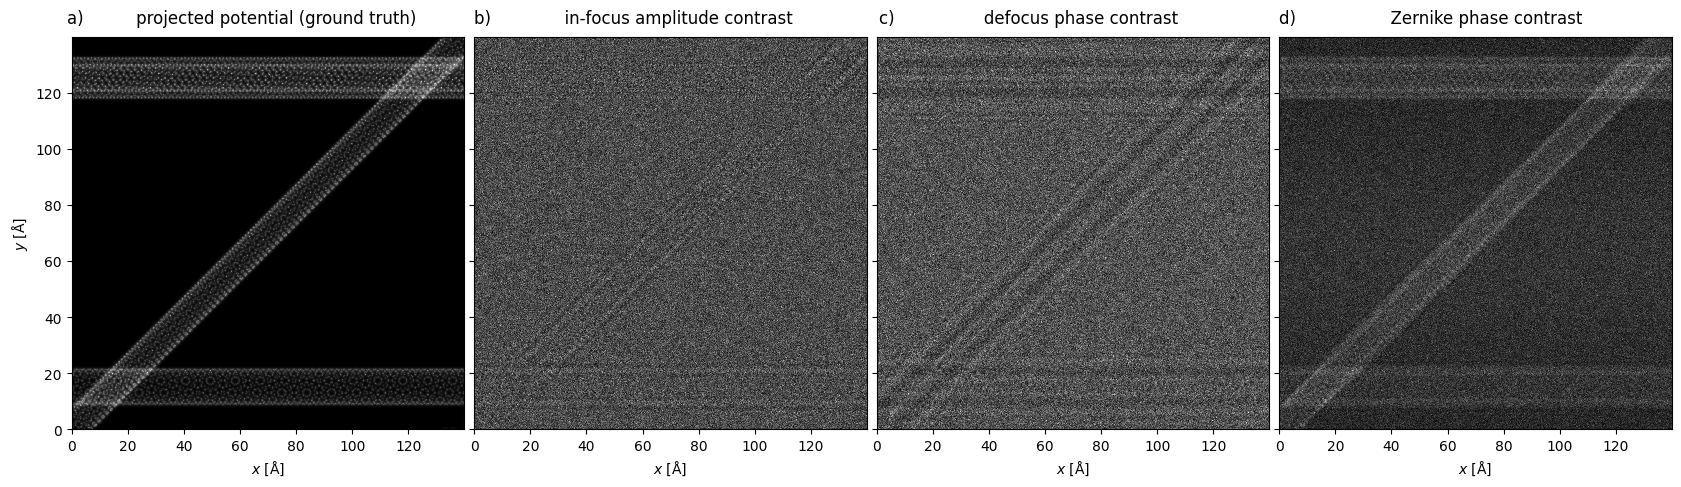
\includegraphics[width=\textwidth]{raster/phase_contrast_imaging_CNTs.png}
  \caption{Simulated high-resolution TEM imaging
  (a)~of single- and double-walled carbon nanotubes, acquired with an electron dose ofv$500~\mathrm{e}/\text{\AA}^2$ using:
  (b)~in-focus optics,
  (c)~$50$~nm of over-focus,
  and (d)~an ideal Zernike phase plate.}
  \label{fig:pci}
\end{figure*}

\subsection{Diffractive Imaging}

As discussed above, STEM is inherently a diffraction-based technique: at each probe position $\boldsymbol{R}$, we have access to the diffraction intensity $I(\boldsymbol{R},\boldsymbol{k}) = \lvert \tilde{\psi}_{\text{exit}}(\boldsymbol{R},\boldsymbol{k}) \rvert^2$, where $\boldsymbol{k}$ is the in-plane scattering vector.
Historically, STEM has used monolithic annular detectors that integrate this intensity within annular collection limits to form a real-space image.
A conventional annular signal is therefore given by
\begin{equation}
  I_{\text{ann}}(\boldsymbol{R}) = \int_{\theta_{\text{in}}}^{\theta_{\text{out}}} I(\boldsymbol{R},\boldsymbol{k})\,\mathrm{d}\boldsymbol{k},
  \label{eq:annular-int}
\end{equation}
yielding familiar contrast modes such as bright-field (BF), annular bright-field (ABF), annular dark-field (ADF), and high-angle annular dark-field (HAADF) STEM~\cite{Crewe_1970,Pennycook_1991}.
Dark-field images in particular are highly interpretable -- especially for crystalline specimens -- leading to their prevalence in materials science characterization~\cite{Ophus_2023}.
However, they discard sensitive information encoded in the exit-wave phase and are often not sufficiently electron-dose efficient for beam-sensitive samples.

The development of fast, low-noise direct-electron detectors~\cite{Levin_2021} has enabled recording the full diffraction pattern $I(\boldsymbol{R},\boldsymbol{k})$ at every scan position, giving rise to a family of techniques collectively known as 4D-STEM~\cite{Ophus_2019}.
These datasets retain the full diffractive signature of the probe–specimen interaction, far beyond what can be accessed with scalar annular signals.
Small convergence-angle (``nanobeam'') and large convergence-angle (diffractive imaging) geometries are shown in \cref{fig:schematic}b-c, respectively.
In this review, we focus on the large class of approaches that computationally recover the phase of the specimen from this set of diffraction patterns, which relies on a large convergence angle (\cref{fig:schematic}c).
We refer to this class of approaches as diffractive imaging or STEM \emph{phase-retrieval} techniques~\cite{sanchez2025}.

\subsubsection{Weak Phase Object Approximation}

Under the WPOA in \cref{eq:wpoa}, the specimen transmission function is $t(\boldsymbol{r}) \approx 1 + i \sigma V_p(\boldsymbol{r})$, with the Fourier transform of the scattered component given by $\tilde{\phi}(\boldsymbol{k}) = \mathcal{F}_{\boldsymbol{r}\rightarrow\boldsymbol{k}}\{t(\boldsymbol{r})\}$.
In this regime, the diffraction intensity can be written as the self-convolution of the converged probe $\tilde{\psi}(\boldsymbol{k})$ with the WPOA term~\cite{Rodenburg_1993}:
\begin{align}
  I(\boldsymbol{R},\boldsymbol{k}) = \iint\, &\tilde{\psi}(\boldsymbol{k}')
  \tilde{\phi}(\boldsymbol{k}-\boldsymbol{k}')
  \tilde{\psi}^{*}(\boldsymbol{k}'')
  \tilde{\phi}^{*}(\boldsymbol{k}-\boldsymbol{k}'') \nonumber \\
  &\times \exp\!\left[2\pi i\,\boldsymbol{R}\cdot(\boldsymbol{k}'-\boldsymbol{k}'')\right]
  \,\mathrm{d}\boldsymbol{k}'\,\mathrm{d}\boldsymbol{k}'' .
  \label{eq:wpoa-intensity}
\end{align}

Following Rodenburg et al.~\cite{Rodenburg_1993}, it is convenient to take the Fourier transform of the measured intensities with respect to the scan position, $G(\boldsymbol{q},\boldsymbol{k}) = \mathcal{F}_{\boldsymbol{R}\rightarrow\boldsymbol{q}}\{I(\boldsymbol{R},\boldsymbol{k})\}$, where $\boldsymbol{q}$ is the reciprocal variable corresponding to the real-space coordinate $\boldsymbol{r}$.
Using the identity $\tilde{\phi}(\boldsymbol{k}) = -\tilde{\phi}^{*}(-\boldsymbol{k})$~\cite{Rodenburg_1993}, one obtains~\cite{Yang_2016}
\begin{align}
  G(\boldsymbol{q},\boldsymbol{k}) &= \lvert \tilde{\psi}(\boldsymbol{k}) \rvert^2 \delta(\boldsymbol{q}) + \Gamma(\boldsymbol{q},\boldsymbol{k})\,\tilde{\phi}(\boldsymbol{q}), \\
  \Gamma(\boldsymbol{q},\boldsymbol{k}) &\equiv \tilde{\psi}^{*}(\boldsymbol{k})\tilde{\psi}(\boldsymbol{k}-\boldsymbol{q}) - \tilde{\psi}(\boldsymbol{k})\tilde{\psi}^{*}(\boldsymbol{k}+\boldsymbol{q}),
  \label{eq:wpoa-forward}
\end{align}
where the aperture overlap function $\Gamma(\boldsymbol{q},\boldsymbol{k})$ encapsulates the probe geometry and forms the basis of all non-iterative STEM phase-retrieval methods.
\cref{fig:gamma} shows characteristic views of $\Gamma(\boldsymbol{q},\boldsymbol{k})$ for a defocused probe with a circular aperture.

We take the probe to have the form $\tilde{\psi}(\boldsymbol{k}) = A(\boldsymbol{k})\,\exp[-i\chi(\boldsymbol{k})]$, where $A(\boldsymbol{k})$ is a top-hat function describing the probe-forming aperture and $\chi(\boldsymbol{k})$ is the aberration surface given by
\begin{equation}
  \chi(\boldsymbol{k}) = \frac{2\pi}{\lambda} \sum_{n,m} \frac{1}{n+1} C_{n,m} (k\lambda)^{n+1} \cos\!\left[m(\theta-\theta_{n,m})\right],
  \label{eq:chi}
\end{equation}
with $k=\lvert\boldsymbol{k}\rvert$, $\theta=\arctan(\boldsymbol{k})$, and $n$ and $m$ the radial and azimuthal orders of the aberration coefficients $C_{n,m}$ with axes $\theta_{n,m}$.

\begin{figure*}[t]
  \centering
  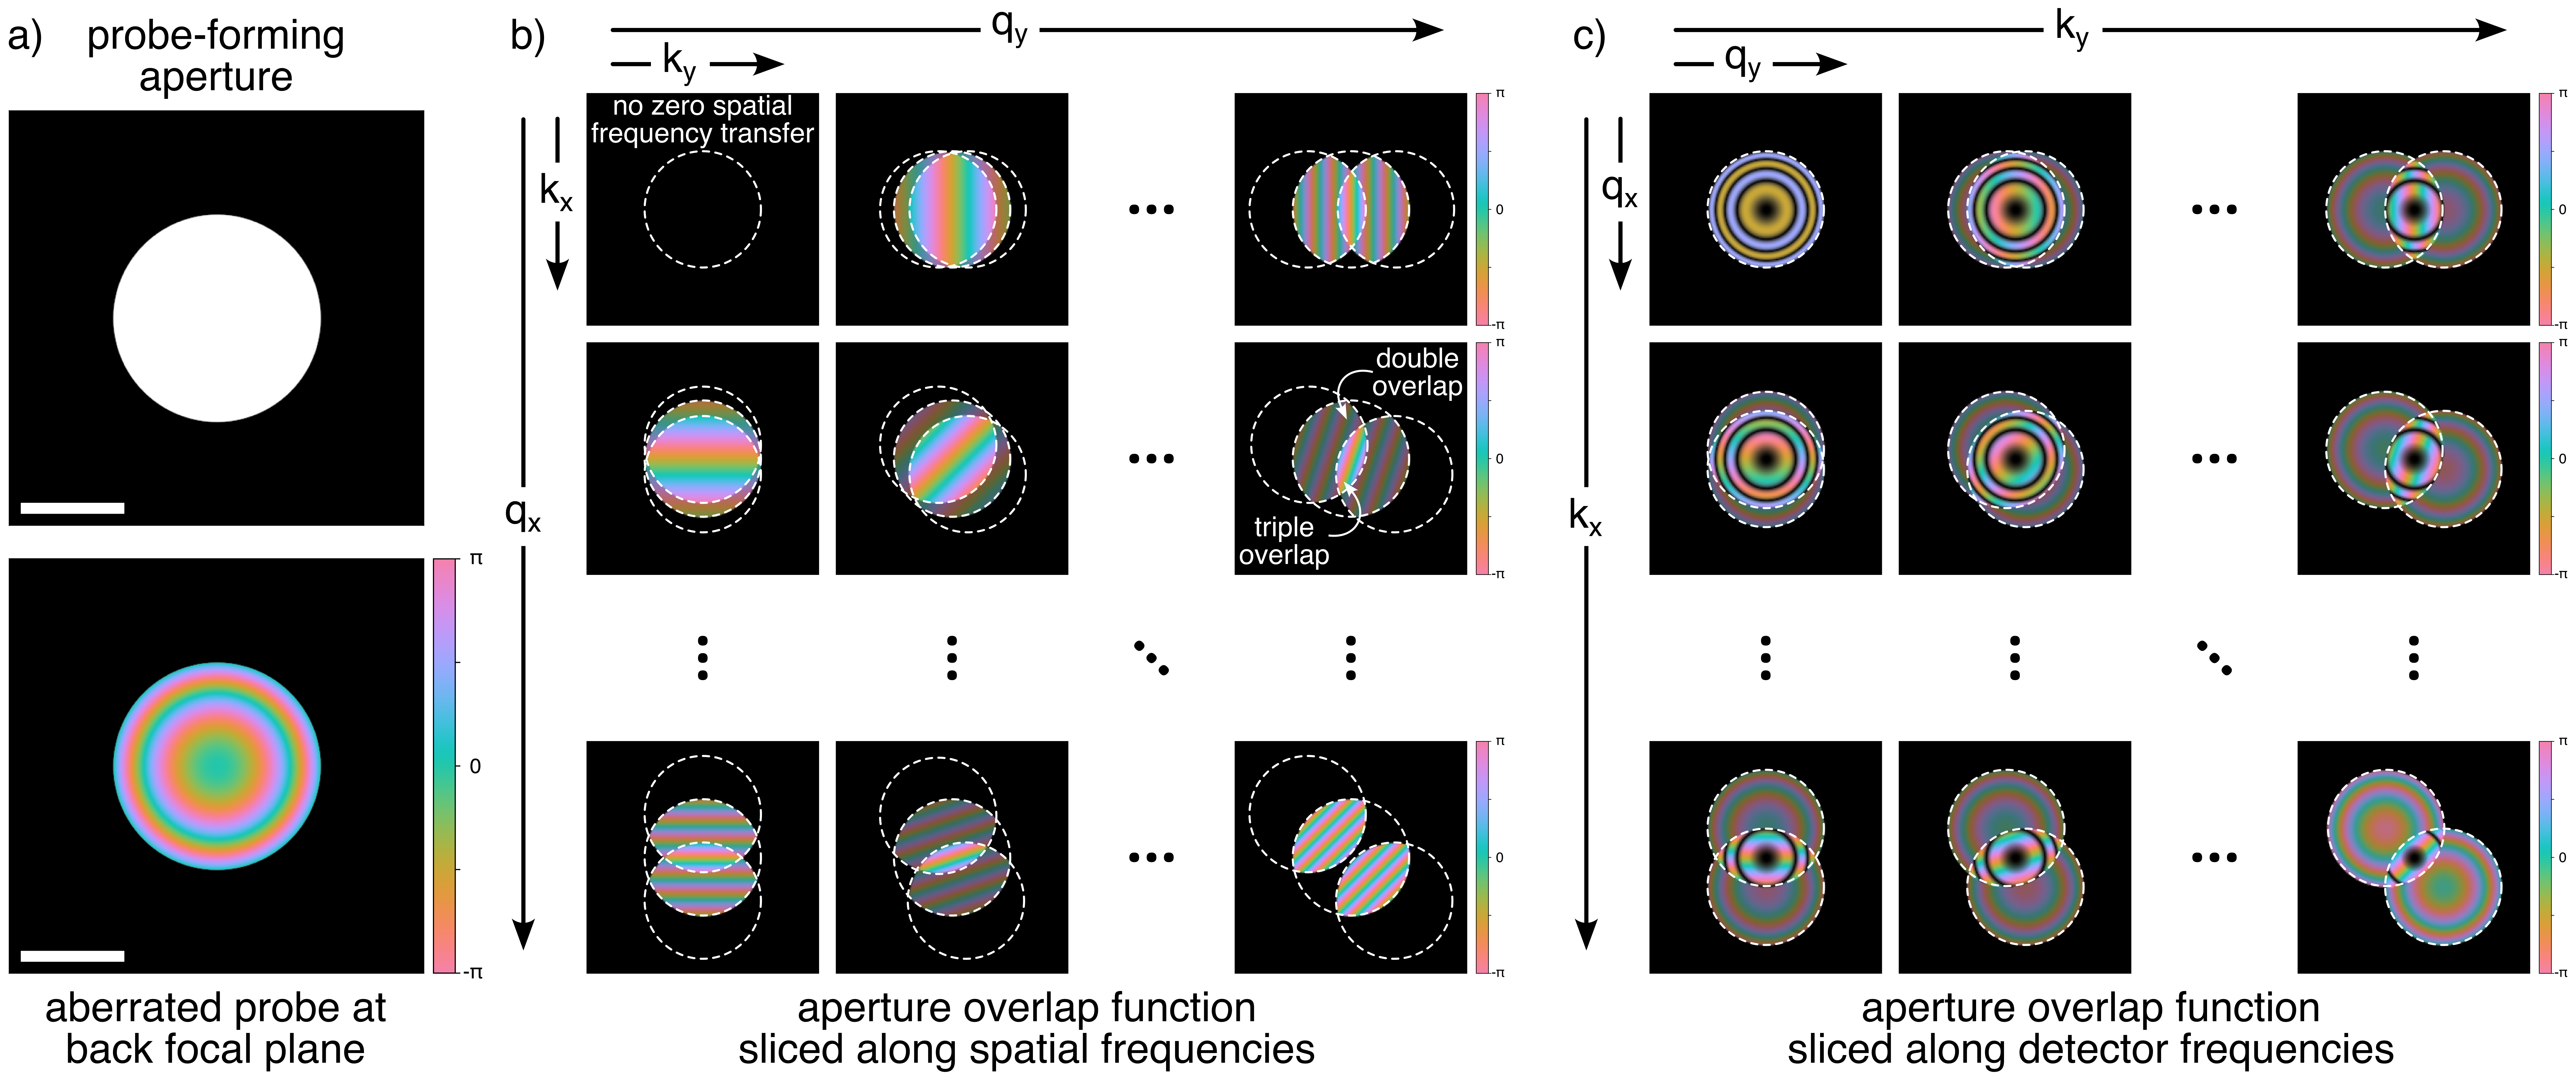
\includegraphics[width=\textwidth]{raster/mrs-bulletin-fig2.png}
  \caption{Components of the aperture overlap function, $\Gamma(\boldsymbol{q},\boldsymbol{k})$.
  (a)~Probe-forming aperture with (bottom) and without (top) aberration function at the back focal plane.
  (b)~Slices along spatial frequencies $\boldsymbol{q}$ plotted over detector frequencies $\boldsymbol{k}$, highlighting the so-called ``double'' and ``triple'' overlap (``trotter'') regions.
  (c)~Slices along detector frequencies $\boldsymbol{k}$ plotted over spatial frequencies $\boldsymbol{q}$, illustrating the effect of shifting the probe aperture and aberrations.}
  \label{fig:gamma}
\end{figure*}

\subsubsection{Transfer of Information}

Under the WPOA, STEM image formation is linear in the specimen phase.
This allows us to define a contrast transfer function, $\mathrm{CTF}(\boldsymbol{q})$, describing how well spatial frequencies of the specimen are transmitted or, in the context of STEM phase-retrieval techniques, how faithfully they can be reconstructed.
We write the reconstructed phase as
\begin{equation}
  \tilde{\psi}_{\text{rec}}(\boldsymbol{q}) = 2\,\tilde{\phi}(\boldsymbol{q})\,\mathrm{CTF}(\boldsymbol{q}),
  \label{eq:recon-ctf}
\end{equation}
where the factor of $2$ follows common conventions~\cite{Dwyer_2024,Vega_2025}.
An ideal phase-retrieval method would therefore satisfy $\mathrm{CTF}_{\text{ideal}}(\boldsymbol{q})=1$.

For an arbitrary detector response function $D_j(\boldsymbol{k})$ (with $j$ indexing a detector pixel or segment), Hammel and Rose~\cite{Hammel_1995} showed that the complex-valued CTF is~\cite{Hammel_1995,rose_1977}
\begin{equation}
  \mathrm{CTF}_j(\boldsymbol{q}) = \frac{i}{2} \int
  \Big[
    D_j(\boldsymbol{k})\,\tilde{\psi}^{*}(\boldsymbol{k})\tilde{\psi}(\boldsymbol{q}-\boldsymbol{k})
    - D_j(\boldsymbol{k})\,\tilde{\psi}(\boldsymbol{k})\tilde{\psi}^{*}(\boldsymbol{q}+\boldsymbol{k})
  \Big]
  \,\mathrm{d}\boldsymbol{k}.
  \label{eq:ctf}
\end{equation}

For a pixelated detector, $D_j(\boldsymbol{k})=\delta(\boldsymbol{k})$, the integrand reduces to the aperture-overlap function $\Gamma(\boldsymbol{q},\boldsymbol{k})$.
More compact expressions follow from an asymmetric decomposition of cross-correlations~\cite{Bekkevold_2025,Lazic_2017}:
\begin{align}
  \Re\{\mathrm{CTF}_j(\boldsymbol{q})\} &= \frac{1}{2}
   \Big(
    [\psi \star (\psi D_j)](\boldsymbol{q})
    +
    [(\psi D_j)\star \psi](\boldsymbol{q})
  \Big),
  \label{eq:ctf-corr-real} \\
  \Im\{\mathrm{CTF}_j(\boldsymbol{q})\} &= \frac{1}{2}
  \Big(
    [\psi \star (\psi D_j)](\boldsymbol{q})
    - [(\psi D_j)\star \psi](\boldsymbol{q})
  \Big),
  \label{eq:ctf-corr-imag}
\end{align}
where $\star$ denotes cross-correlation and $\Re\{\cdot\}$ and $\Im\{\cdot\}$ represent real and imaginary components.

Two limiting cases of \cref{eq:ctf} provide further physical insight.
In the absence of aberrations, $\chi(\boldsymbol{k})=0$, the real part of \cref{eq:ctf-corr-real} vanishes and the imaginary part reduces to the aperture autocorrelation:
\begin{align}
  \mathrm{CTF}_{\text{in-focus}}(\boldsymbol{q}) &= i\,[A\star A](\boldsymbol{q}) \nonumber \\
  &= i\,\Re\!\left\{ \mathcal{F}^{-1}_{\boldsymbol{r}\rightarrow\boldsymbol{q}} \left[ \left| \mathcal{F}_{\boldsymbol{q}\rightarrow\boldsymbol{r}}\{A(\boldsymbol{q})\} \right|^2 \right] \right\}.
  \label{eq:infocus-ctf}
\end{align}
This envelope is a fundamental limit for all non-iterative STEM phase-retrieval methods.

Similarly, evaluating \cref{eq:ctf} for the axial-illumination case, $\boldsymbol{k}=0$, yields a purely imaginary CTF:
\begin{equation}
  \mathrm{CTF}_{\text{axial}}(\boldsymbol{q}) = - i\,\sin\!\big[\chi(\boldsymbol{q})\big],
  \label{eq:ctf-axial}
\end{equation}
which is precisely the HRTEM CTF derived in the previous section, illustrating the \emph{principle of reciprocity} between TEM and STEM techniques~\cite{Williams_2009,Carter_2016,Kirkland_2020}.

\subsubsection{Statistically Reliable Information}

The CTF describes only the maximum transferable signal, not the statistical reliability of that signal in the presence of noise.
A complete description of information transfer must account for noise statistics, notably shot noise in electron detectors.
The natural figure of merit is the spectral signal-to-noise ratio (SSNR)~\cite{Unser_1987,Varnavides_2025_ssnr},
\begin{equation}
  \mathrm{SSNR}(\boldsymbol{q}) = \frac{\lvert \langle \tilde{\psi}(\boldsymbol{q}) \rangle \rvert} {\sqrt{\operatorname{Var}\!\left[\tilde{\psi}(\boldsymbol{q})\right]}},
  \label{eq:ssnr}
\end{equation}
which quantifies the statistically reliable recoverable information at each spatial frequency.

The SSNR is related to the detective quantum efficiency (DQE), recently introduced as a quantitative performance metric for STEM phase retrieval~\cite{Bennemann_2025}:
\begin{equation}
  \mathrm{DQE}(\boldsymbol{q}) = \frac{\mathrm{SSNR}_{\text{out}}^{2}(\boldsymbol{q})} {\mathrm{SSNR}_{\text{in}}^{2}(\boldsymbol{q})},
  \label{eq:dqe}
\end{equation}
where $\mathrm{SSNR}_{\text{in}}(\boldsymbol{q})$ is the SSNR of an ``ideal'' reference system, typically taken as HRTEM with a Zernike phase plate~\cite{Zernike_1942,Vega_2025}.
Thus, the DQE provides a normalized measure of how efficiently a method transfers information relative to a theoretical optimum.

\section{Direct Phase Retrieval Techniques}

Equipped with the WPOA aperture-overlap and CTF/SSNR formalisms, we are now ready to investigate the zoo of non-iterative STEM phase-retrieval methods and their various acronyms.
These differ primarily in how they combine the Fourier-transformed measured diffraction intensities $G(\boldsymbol{q},\boldsymbol{k})$ to produce an estimate for the specimen phase $\tilde{\phi}(\boldsymbol{q})$.

\subsection{Phase-Compensated Coherent Sum}
\label{sec:ssb}

The first technique we investigate goes by two seemingly unrelated names: \emph{aberration-corrected bright-field (acBF) STEM}~\cite{Ma_2025} and \emph{phase-compensated single-sideband (SSB) ptychography}~\cite{Yang_2016}.
The former highlights its close connection to \emph{tilt-corrected bright-field (tcBF) STEM}, which we investigate further in the Quadratic Approximation section.
The latter name reflects the structure of the WPOA forward model in \cref{eq:wpoa-forward}, which contains two redundant contributions at $\boldsymbol{q}$ and $-\boldsymbol{q}$.

In the absence of aberrations, these two ``sidebands'' are related by complex conjugation according to Friedel's law.\footnote{Friedel's law illustrates how a single mathematical principle -- the Hermitian conjugation symmetry of the Fourier transform of a real-valued function -- connects the physics of imaging with crystallographic structure determination~\cite{Friedel_1913,karle1985}.}
Accordingly, the specimen phase $\tilde{\phi}(\boldsymbol{q})$ can be reconstructed using only one of them.
In practice, once aberrations are present, the two sidebands are no longer perfect conjugates: residual aberrations imprint an additional geometric phase on the aperture-overlap function $\Gamma(\boldsymbol{q},\boldsymbol{k})$.

The key insight behind SSB is that, under the WPOA, detector pixels sampling the same sideband carry the same specimen phase $\tilde{\phi}(\boldsymbol{q})$.
Differences between pixels arise only from known, instrument-dependent phases, namely aberration-induced geometric phases and aperture-overlap geometry.
If these extra phases are removed, sideband contributions from all detector pixels can be added coherently.

Phase-compensated SSB accomplishes this by dividing $\Gamma(\boldsymbol{q},\boldsymbol{k})$ by its magnitude and retaining only its phase factor, effectively rotating each detector-plane frequency into a common phase reference.
The estimated phase is then obtained by coherently summing all phase-aligned detector samples~\cite{Yang_2016}:
\begin{equation}
  \tilde{\phi}_{\text{SSB}}(\boldsymbol{q}) = \sum_{\boldsymbol{k}} \frac{\Gamma^{*}(\boldsymbol{q},\boldsymbol{k})\,G(\boldsymbol{q},\boldsymbol{k})} {\lvert \Gamma(\boldsymbol{q},\boldsymbol{k}) \rvert}.
  \label{eq:ssb-recon}
\end{equation}

\Cref{eq:ssb-recon} works remarkably well and remains one of the most widely used direct phase-retrieval techniques.
Inserting the forward model $G(\boldsymbol{q},\boldsymbol{k})=\Gamma(\boldsymbol{q},\boldsymbol{k})\tilde{\phi}(\boldsymbol{q})$ into \cref{eq:ssb-recon} gives the SSB CTF~\cite{Yang_2016}
\begin{equation}
  \mathrm{CTF}_{\text{SSB}}(\boldsymbol{q}) = \frac{i}{2} \sum_{\boldsymbol{k}} \lvert \Gamma(\boldsymbol{q},\boldsymbol{k}) \rvert.
  \label{eq:ctf-ssb}
\end{equation}
For spatial frequencies beyond the aperture semiangle, $\lvert \boldsymbol{q} \rvert > q_0$, the overlap $\Gamma(\boldsymbol{q},\boldsymbol{k})$ reduces to the double-overlap region, and the CTF collapses to the ideal autocorrelation envelope in \cref{eq:infocus-ctf}.

To understand the SSB variance, note that each detector frequency contributes a noisy measurement,
\begin{equation}
  G(\boldsymbol{q},\boldsymbol{k}) = \Gamma(\boldsymbol{q},\boldsymbol{k})\tilde{\phi}(\boldsymbol{q}) + n(\boldsymbol{q},\boldsymbol{k}),
  \label{eq:noise-model}
\end{equation}
with unit-variance noise $n(\boldsymbol{q},\boldsymbol{k})$~\cite{Bennemann_2025}.
The phase-alignment step preserves unit variance, so noise contributions add incoherently while the signal adds coherently.
Thus, the total variance at each spatial frequency $\boldsymbol{q}$ is simply the number of detector pixels for which $\Gamma(\boldsymbol{q},\boldsymbol{k})$ is nonzero:
\begin{align}
  \operatorname{Var}\!\left[\tilde{\phi}_{\text{SSB}}(\boldsymbol{q})\right] &= \sum_{\boldsymbol{k}} \mathbf{1}_{\{\lvert \Gamma(\boldsymbol{q},\boldsymbol{k}) \rvert > 0\}} \nonumber\\
  &= 2 D(\boldsymbol{q})+T(\boldsymbol{q}), 
  \label{eq:var-ssb}
\end{align}
where $D(\boldsymbol{q})$ and $T(\boldsymbol{q})$ are the double- and triple-overlap regions (\cref{fig:gamma}).
The resulting SSNR is~\cite{Bennemann_2025,Varnavides_2025_ssnr}
\begin{equation}
  \mathrm{SSNR}_{\text{SSB}}(\boldsymbol{q}) = \frac{\sum_{\boldsymbol{k}}\lvert \Gamma(\boldsymbol{q},\boldsymbol{k}) \rvert} {2\sqrt{2D(\boldsymbol{q})+T(\boldsymbol{q})}} .
  \label{eq:ssb-ssnr}
\end{equation}

\subsection{Noise-Flattening Normalization}
\label{sec:obf}

Phase-compensated SSB improves robustness against residual aberrations by removing the geometric phase of the aperture-overlap function before summing detector-plane frequencies.
However, SSB still treats all contributing detector pixels equally, even though the strength of the aperture overlap varies strongly across the bright-field disk, resulting in a statistically sub-optimal reconstruction.

The \emph{optimum bright-field (OBF) STEM} method addresses this by applying a noise-matched normalization to the SSB estimator~\cite{Ooe_2021,Ooe_2024}.
Starting from the phase-aligned numerator, OBF introduces a scalar normalization factor proportional to the root-mean-squared aperture-overlap strength:
\begin{equation}
  \tilde{\phi}_{\text{OBF}}(\boldsymbol{q}) = \frac{\sum_{\boldsymbol{k}} \Gamma^{*}(\boldsymbol{q},\boldsymbol{k})\,G(\boldsymbol{q},\boldsymbol{k})} {\sqrt{\sum_{\boldsymbol{k}}\lvert \Gamma(\boldsymbol{q},\boldsymbol{k}) \rvert^2}} .
  \label{eq:obf-recon}
\end{equation}

The denominator rescales the coherent SSB sum by the effective SSNR of the bright-field detector region.
For each spatial frequency, this normalization prevents a small subset of bright-field pixels with weak overlap from amplifying noise.
Thus, OBF can be viewed as a noise-flattened SSB formulation, retaining geometric phase compensation but adjusting its gain to reflect information reliability.

Substituting the WPOA forward model into \cref{eq:obf-recon} gives
\begin{equation}
  \mathrm{CTF}_{\text{OBF}}(\boldsymbol{q}) = \frac{i}{2} \sqrt{\sum_{\boldsymbol{k}}\lvert \Gamma(\boldsymbol{q},\boldsymbol{k}) \rvert^2}.
  \label{eq:obf-ctf}
\end{equation}

Using the additive unit-variance noise model in \cref{eq:noise-model}, the numerator becomes
\begin{align}
  \sum_{\boldsymbol{k}}\Gamma^{*}(\boldsymbol{q},\boldsymbol{k})G(\boldsymbol{q},\boldsymbol{k}) &=
  \sum_{\boldsymbol{k}}\lvert \Gamma(\boldsymbol{q},\boldsymbol{k}) \rvert^2 \tilde{\phi}(\boldsymbol{q}) \nonumber\\
  &\quad + \sum_{\boldsymbol{k}}\Gamma^{*}(\boldsymbol{q},\boldsymbol{k})n(\boldsymbol{q},\boldsymbol{k}),
  \label{eq:obf-numerator}
\end{align}
with variance
\begin{equation}
  \operatorname{Var}\!\left[ \sum_{\boldsymbol{k}}\Gamma^{*}(\boldsymbol{q},\boldsymbol{k})n(\boldsymbol{q},\boldsymbol{k}) \right] = \sum_{\boldsymbol{k}}\lvert \Gamma(\boldsymbol{q},\boldsymbol{k}) \rvert^2 .
  \label{eq:obf-var}
\end{equation}
This is precisely the OBF denominator squared, thus normalizing the OBF variance to unity, $\operatorname{Var}[\tilde{\phi}_{\text{OBF}}(\boldsymbol{q})]=1$.
The resulting OBF SSNR is thus given simply by the magnitude of its CTF
\begin{equation}
  \mathrm{SSNR}_{\text{OBF}}(\boldsymbol{q}) = \frac{1}{2} \sqrt{\sum_{\boldsymbol{k}}\lvert \Gamma(\boldsymbol{q},\boldsymbol{k}) \rvert^2}.
  \label{eq:obf-ssnr}
\end{equation}

\begin{figure*}[t]
  \centering
  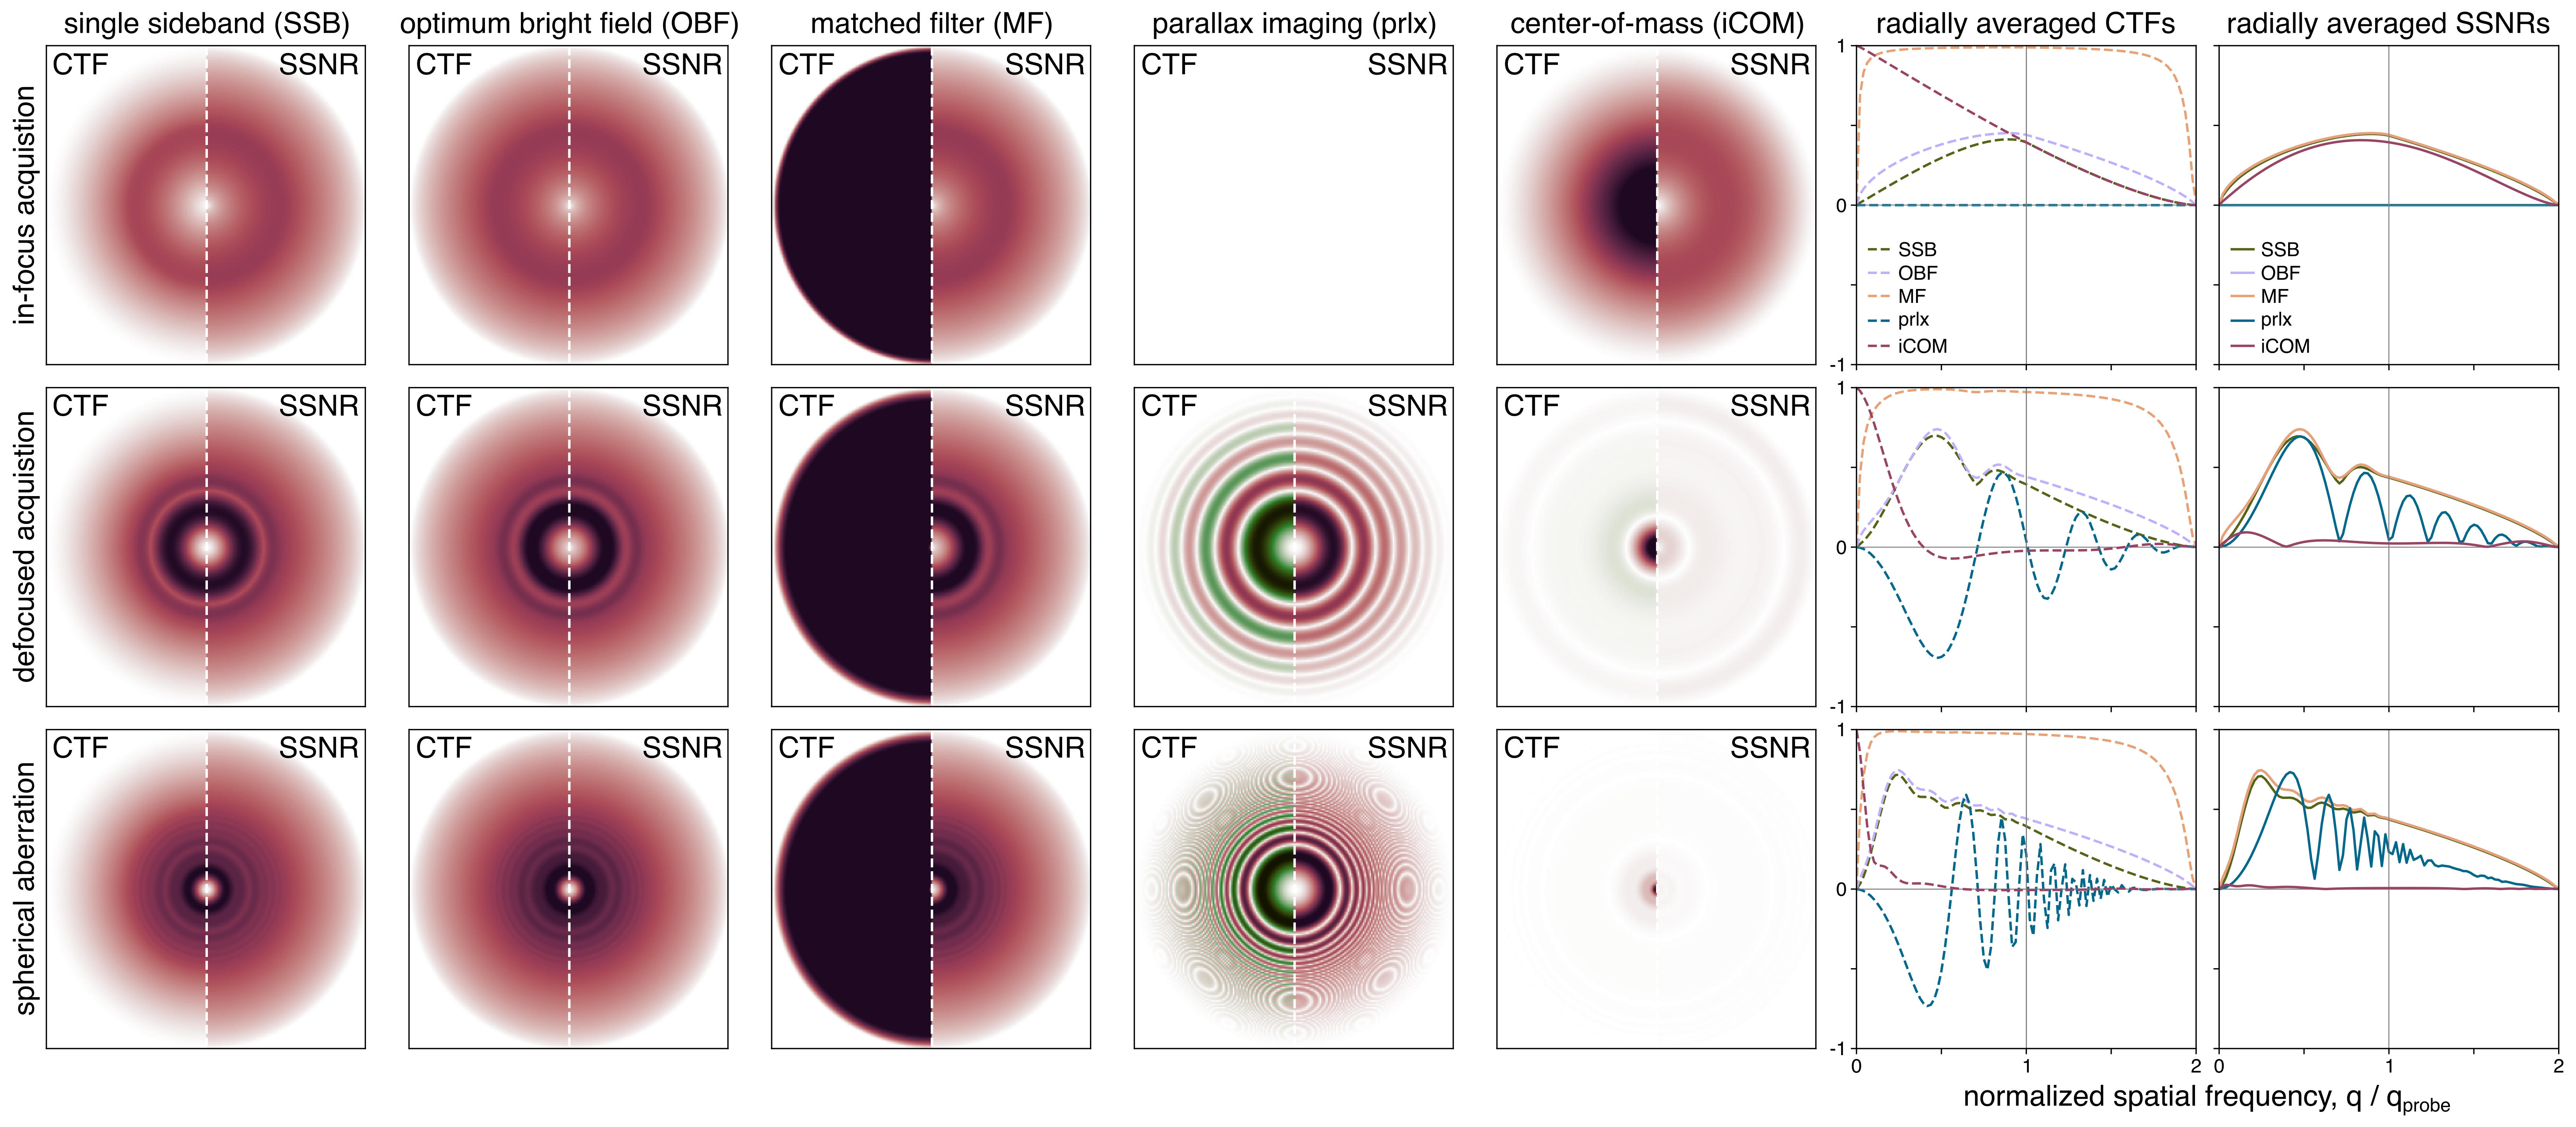
\includegraphics[width=\textwidth]{raster/direct-ctf-figure.png}
  \caption{Contrast transfer functions (CTFs) and spectral signal-to-noise ratios (SSNRs) for all direct techniques investigated across different acquisition parameters, highlighting the SSNR equivalence for SSB, OBF, and MF/WDD.}
  \label{fig:ctf}
\end{figure*}

\subsection{Least-Squares Matched Filter}
\label{sec:wdd}

The OBF estimator above improves SSB by normalizing the coherent sum, but it is not formally a least-squares estimator.
The proper matched-filter (MF) solution for recovering $\tilde(\phi)(\boldsymbol{q})$ from the WPOA forward model is obtained by minimizing $\sum_{\boldsymbol{k}}\lvert G(\boldsymbol{q},\boldsymbol{k})-\Gamma(\boldsymbol{q},\boldsymbol{k})\tilde{\phi}(\boldsymbol{q}) \rvert^2$, yielding the estimator
\begin{equation}
  \tilde{\phi}_{\text{MF}}(\boldsymbol{q}) = 
  \frac{\sum_{\boldsymbol{k}} \Gamma^{*}(\boldsymbol{q},\boldsymbol{k})\,G(\boldsymbol{q},\boldsymbol{k})}
  {\sum_{\boldsymbol{k}}\lvert \Gamma(\boldsymbol{q},\boldsymbol{k}) \rvert^2 + \epsilon(\boldsymbol{q})}.
  \label{eq:mf-recon}
\end{equation}

While \cref{eq-mf-recon} is simple, direct evaluation in detector-space is numerically unstable:
the numerator contains highly oscillatory phases from $\Gamma(\boldsymbol{q},\boldsymbol{k})$, and the denominator depends on the squared magnitude of a rapidly varying overlap kernel.
Applying Parseval's theorem, $\sum_k \lvert \tilde(f)(k)\rvert^2 = \int d r \lvert f(r)\rvert^2$, and inverse Fourier transforming over $\boldsymbol{k}$ gives the MF estimator in the mixed-domain representation
\begin{align}
\tilde{\phi}_{\text{MF-mix}}(\boldsymbol{q})
&=
\frac{\int W^{*}(\boldsymbol{q},\boldsymbol{\rho})H(\boldsymbol{q},\boldsymbol{\rho})\,\mathrm{d}\boldsymbol{\rho}}
{\int \lvert W(\boldsymbol{q},\boldsymbol{\rho}) \rvert^2\,\mathrm{d}\boldsymbol{\rho}+\epsilon(\boldsymbol{q})},
\label{eq:mf-mixed-recon}
\\
W(\boldsymbol{q},\boldsymbol{\rho})
&=
\mathcal{F}^{-1}\{\Gamma(\boldsymbol{q},\boldsymbol{k})\},
\label{eq:wigner-w}
\\
H(\boldsymbol{q},\boldsymbol{\rho})
&=
\mathcal{F}^{-1}\{G(\boldsymbol{q},\boldsymbol{k})\},
\label{eq:wigner-h}
\end{align}
leading to the Wigner distribution deconvolution (WDD) estimator~\cite{Rodenburg_1992,Li_2014,Yang_2017}.

The MF/WDD CTF is
\begin{equation}
\mathrm{CTF}_{\text{MF}}(\boldsymbol{q})
=
\frac{\sum_{\boldsymbol{k}}\lvert \Gamma(\boldsymbol{q},\boldsymbol{k}) \rvert^2}
{\sum_{\boldsymbol{k}}\lvert \Gamma(\boldsymbol{q},\boldsymbol{k}) \rvert^2+\epsilon(\boldsymbol{q})},
\label{eq:mf-ctf}
\end{equation}
with variance
\begin{equation}
\operatorname{Var}\!\left[\tilde{\phi}_{\text{MF}}(\boldsymbol{q})\right]
=
\frac{1}{\sum_{\boldsymbol{k}}\lvert \Gamma(\boldsymbol{q},\boldsymbol{k}) \rvert^2},
\label{eq:mf-var}
\end{equation}
yielding an SSNR identical to OBF:
\begin{equation}
\mathrm{SSNR}_{\text{MF}}(\boldsymbol{q})
=
\frac{1}{2}
\sqrt{\sum_{\boldsymbol{k}}\lvert \Gamma(\boldsymbol{q},\boldsymbol{k}) \rvert^2}.
\label{eq:mf-ssnr}
\end{equation}

\begin{figure*}[t]
  \centering
  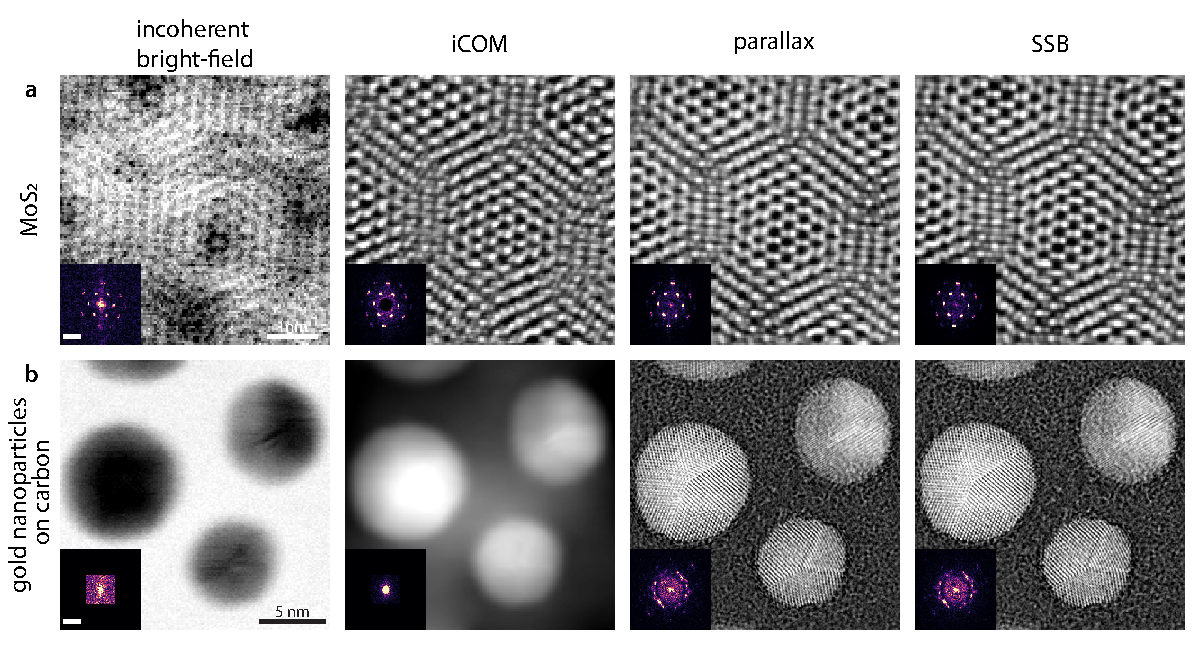
\includegraphics[width=\textwidth]{vector/direct_gold_mos2.pdf}
  \caption{Direct-method reconstructions for (a)~near-focus MoS$_2$ acquisition~\cite{zhang2025atom} and (b)~defocused gold nanoparticle datasets.}
  \label{fig:exp-compare}
\end{figure*}

\subsection{Quadratic Approximation} \label{sec:parallax}

Parallax imaging (tcBF) provides a computationally efficient approximation to SSB~\cite{Nguyen_2016,Spoth_2017,Yu_2025,Varnavides_2023,Varnavides_2024,Varnavides_2025}.
Taylor-expanding $\Gamma(\boldsymbol{q},\boldsymbol{k})$ to first order in $\boldsymbol{q}$ gives
\begin{align}
\Gamma(\boldsymbol{q},\boldsymbol{k})
&\approx
\beta(\boldsymbol{q},\boldsymbol{k})
\exp\!\left[i\nabla_{\boldsymbol{k}}\chi(\boldsymbol{k})\cdot\boldsymbol{q}\right],
\\
\beta(\boldsymbol{q},\boldsymbol{k})
&=
A(\boldsymbol{k})
\Big[
A(\boldsymbol{q}-\boldsymbol{k})e^{-i\chi(\boldsymbol{q})}
-
A(\boldsymbol{q}+\boldsymbol{k})e^{i\chi(\boldsymbol{q})}
\Big].
\label{eq:prlx-gamma-approx}
\end{align}

The parallax estimator is
\begin{equation}
\tilde{\phi}_{\text{prlx}}(\boldsymbol{q})
=
\sum_{\boldsymbol{k}}
G(\boldsymbol{q},\boldsymbol{k})
\,\operatorname{sgn}[\sin\chi(\boldsymbol{q})]\,
e^{-i\nabla_{\boldsymbol{k}}\chi(\boldsymbol{k})\cdot\boldsymbol{q}} .
\label{eq:par-recon}
\end{equation}

Its CTF is
\begin{align}
\mathrm{CTF}_{\text{prlx}}(\boldsymbol{q})
&=
\frac{i}{2}\sum_{\boldsymbol{k}}\beta(\boldsymbol{q},\boldsymbol{k})
\nonumber\\
&=
-i\,\sin[\chi(\boldsymbol{q})]\,[A\star A](\boldsymbol{q}),
\label{eq:prlx-ctf}
\end{align}
with SSNR
\begin{equation}
\mathrm{SSNR}_{\text{prlx}}(\boldsymbol{q})
=
\lvert \sin[\chi(\boldsymbol{q})] \rvert\,[A\star A](\boldsymbol{q}).
\label{eq:prlx-ssnr}
\end{equation}

\subsection{First-Moment Projection}
\label{sec:icom}

Integrated center-of-mass (iCOM) or iDPC imaging~\cite{Dekkers_1974,Lazic_2016} uses the first moment of the aperture overlap.
With vector detector response $D(\boldsymbol{k})=\boldsymbol{k}$,
\begin{align}
\mathrm{CTF}_{\text{COM}}(\boldsymbol{q})
&=
\frac{i}{2}\int \Gamma(\boldsymbol{q},\boldsymbol{k})\,\boldsymbol{k}\,\mathrm{d}\boldsymbol{k}
\nonumber\\
&=
\frac{i\boldsymbol{q}}{2}[\tilde{\psi}\star\tilde{\psi}](\boldsymbol{q}).
\label{eq:com-ctf}
\end{align}

Fourier integration yields
\begin{equation}
\tilde{\phi}_{\text{iCOM}}(\boldsymbol{q})
=
\frac{\sum_{\boldsymbol{k}}\boldsymbol{q}\cdot[G(\boldsymbol{q},\boldsymbol{k})\,\boldsymbol{k}]}
{i\lvert \boldsymbol{q} \rvert^2},
\label{eq:icom-recon}
\end{equation}
with scalar CTF
\begin{equation}
\mathrm{CTF}_{\text{iCOM}}(\boldsymbol{q})
=
i[\tilde{\psi}\star\tilde{\psi}](\boldsymbol{q}).
\label{eq:icom-ctf}
\end{equation}

The corresponding SSNR scales as~\cite{Varnavides_2025_ssnr}
\begin{equation}
\mathrm{SSNR}_{\text{iCOM}}(\boldsymbol{q})
=
\frac{\lvert [\tilde{\psi}\star\tilde{\psi}](\boldsymbol{q}) \rvert}
{\lvert \boldsymbol{q} \rvert}.
\label{eq:icom-ssnr}
\end{equation}

\subsection{Comparison of Direct Techniques}

The phase estimators introduced above—SSB, OBF, MF/WDD, parallax, and iCOM—all originate from the same WPOA forward model in \cref{eq:wpoa-forward} and additive noise model in \cref{eq:noise-model}.
They primarily differ in (i) how they weight the bright-field intensities, (ii) how they normalize the coherent sum, and (iii) how much of the aperture-overlap kernel they retain.

SSB performs an unnormalized coherent projection using the full aperture-overlap kernel.
OBF applies a noise-flattening scalar normalization.
MF/WDD implements the least-squares matched filter, either in detector space (MF) or in a mixed domain (WDD).
Parallax imaging uses a first-order approximation to the aperture-overlap kernel, keeping only the detector-frequency-dependent phase ramp
\(
\exp\!\left[i \nabla_{\boldsymbol{k}}\chi(\boldsymbol{k}) \cdot \boldsymbol{q}\right],
\)
making it computationally cheap.
Parallax subpixel shift estimation accuracy enables scan step-size upsampling (\cref{fig:uspsample}), although this can be extended to other direct methods as well~\cite{Varnavides_2025}.
Finally, iCOM bypasses the overlap kernel entirely, and instead takes the first moment of the bright-field intensities and reconstructs the phase by Fourier integration of the resulting COM signal.

\begin{figure}
  \centering
  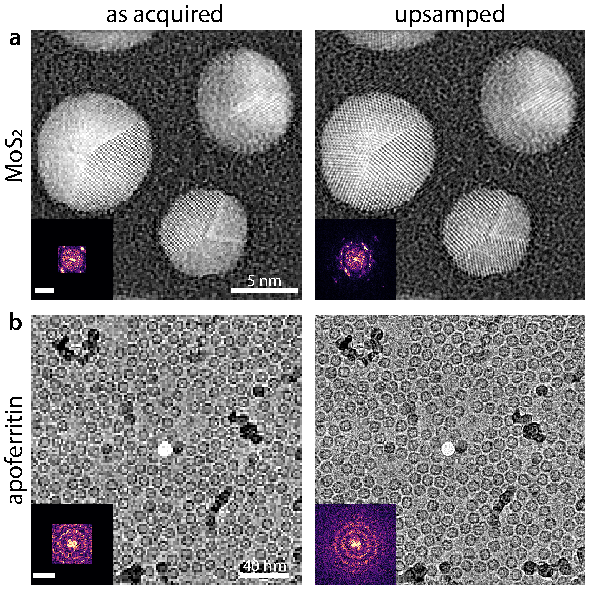
\includegraphics[width=\linewidth]{vector/upsample.pdf}
  \caption{Upsampled
  \textit{(a)} gold nanoparticles and \textit{(b)} apoferritin~\cite{Berk_2024} parallax imaging reconstructions.}
  \label{fig:uspsample}
\end{figure}

With the exception of iCOM, these techniques rely on an accurate estimation of the aberrations, which can be calculated through optimization routines based on self-consistency error~\cite{Varnavides_2025}, or by least-squares fitting of linear systems of equations~\cite{Varnavides_2023,Yu_2025}.

\Cref{unified-pseudocode} shows a unified pseudocode for the direct estimators we have seen so far, using a loop over bright-field pixels $\boldsymbol{k}_{\mathrm{BF}}$.
This leverages the fact that the aperture-overlap function is identically zero outside the probe aperture, making it computationally efficient, and enabling natural upsampling via Fourier tiling~\cite{Varnavides_2025}.
It should be noted that, due to the mixed-domain requirement, WDD cannot be computed by solely looping over $\boldsymbol{k}_{\mathrm{BF}}$.

As highlighted in \cref{fig:ctf,fig:exp-compare}, the ideal approach depends on the nature of the data and acquisition parameters.
For in-focus experiments, iCOM is often the preferred approach, with the low computational overhead of this technique making it most compatible with \textit{in situ} approaches~\cite{bekkevold2024ultra}.
Conversely, parallax reconstructions are often performed for defocused acquisitions using large step sizes, e.g., for beam-sensitive biological samples~\cite{Berk_2024,Yu_2025}.

The SSB, OBF, and MF/WDD techniques perform a full deconvolution of the aperture overlap and are also suited for acquisitions with residual higher-order aberration~\cite{Varnavides_2025,Susi_2025}.
However, ptychographic acquisitions on aberration-corrected instruments are often dominated by first-order aberrations such as defocus and astigmatism, suggesting the quadratic approximation provided by parallax yields a nearly identical reconstruction as SSB, OBF, or MF/WDD~\cite{Varnavides_2025_ssnr}.

\begin{figure}
\renewcommand{\figurename}{Algorithm}
\hrule \vspace{5pt}
\caption{Unified direct STEM phase retrieval}
\vspace{5pt} \hrule \vspace{5pt}
\label{unified-pseudocode}
\begin{algorithmic}

\Statex \textbf{Inputs:}
\Statex \quad 4D-STEM dataset $I(\boldsymbol{r},\boldsymbol{k})$
\Statex \quad estimator type $\in\{\text{SSB},\text{OBF},\text{MF},\text{prlx},\text{iCOM}\}$
\Statex \quad integer upsampling factor $f$
\Statex \quad aberration coefficients $C_{n,m}$ (for $\chi$ and $\nabla_{\boldsymbol{k}}\chi$)
\Statex \quad convergence semiangle $k_0$
\Statex \quad scan/detector rotation angle $\theta$

\Statex \textbf{Output:} estimated phase upsampled by factor $f$

\Statex
\Statex \textbf{Initialization:}
\Statex Allocate $f$-upsampled output array $I'(\boldsymbol{r}') \leftarrow 0$
\Statex Define bright-field index set $\boldsymbol{k}_{\mathrm{BF}}=\{\boldsymbol{k}:|\boldsymbol{k}|<k_0\}$
\Statex Extract bright-field stack $I_{\mathrm{BF}}=\{I(\boldsymbol{r},\boldsymbol{k}):|\boldsymbol{k}|<k_0\}$
\Statex Construct upsampled and $\theta$-rotated frequency grid $\boldsymbol{q}'$

\Statex
\Statex \textbf{Reconstruction:}
\For{$i=1$ to $N_{\mathrm{BF}}$}
  \Statex $G(\boldsymbol{q}) \leftarrow \mathcal{F}_{\boldsymbol{r}\rightarrow\boldsymbol{q}}\!\left[I_{\mathrm{BF}}[i](\boldsymbol{r})\right]$
  \Statex $G(\boldsymbol{q}') \leftarrow \mathrm{tile}_f\!\left[G(\boldsymbol{q})\right]$

  \Statex Compute estimator kernel $H(\boldsymbol{q}')$:
  \Statex \quad SSB:\quad $H=-i\,\Gamma^*(\boldsymbol{q}',\boldsymbol{k}_{\mathrm{BF}})/|\Gamma|$
  \Statex \quad OBF:\quad $H=-i\,\Gamma^*/\sqrt{\sum_{\boldsymbol{k}\in\boldsymbol{k}_{\mathrm{BF}}}|\Gamma|^2}$
  \Statex \quad MF:\quad $H=-i\,\Gamma^*/\left(\sum_{\boldsymbol{k}\in\boldsymbol{k}_{\mathrm{BF}}}|\Gamma|^2+\epsilon(\boldsymbol{q}')\right)$
  \Statex \quad prlx:\quad $H=\exp[-i\nabla_{\boldsymbol{k}}\chi(\boldsymbol{k}_{\mathrm{BF}})\!\cdot\!\boldsymbol{q}']\,\mathrm{sgn}[\sin\chi(\boldsymbol{q}')]$
  \Statex \quad iCOM:\quad $H=-i\,\boldsymbol{k}_{\mathrm{BF}}\!\cdot\!\boldsymbol{q}'/|\boldsymbol{q}'|^2$

  \Statex $I'(\boldsymbol{r}') \mathrel{+}= \Re\!\left\{\mathcal{F}^{-1}_{\boldsymbol{q}'\rightarrow\boldsymbol{r}'}[G(\boldsymbol{q}')H(\boldsymbol{q}')]\right\}/N_{\mathrm{BF}}$
\EndFor

\end{algorithmic}
\vspace{5pt} \hrule
\end{figure}


\bibliographystyle{apsrev4-2}
\bibliography{references}

\end{document}
